\documentclass[aspectratio=169,11pt]{beamer}

% ============================================================
% PACKAGES
% ============================================================
\usepackage{graphicx}
\usepackage{tikz}
\usetikzlibrary{positioning,arrows.meta}
\usepackage{xcolor}
\usepackage{booktabs}
\usepackage{tabularx}
\usepackage{array}
\usepackage{ragged2e}
\usepackage{hyperref}

% ============================================================
% COLORS - SAME AS PHASE-I
% ============================================================
\definecolor{GEUBlue}{RGB}{20,55,105}
\definecolor{GEULightBlue}{RGB}{238,244,251}
\definecolor{GEUGrey}{RGB}{90,90,90}
\definecolor{GEULightGrey}{RGB}{245,246,248}

% ============================================================
% BEAMER SETTINGS
% ============================================================
\usetheme{default}
\setbeamertemplate{navigation symbols}{}
\setbeamertemplate{blocks}[rounded][shadow=false]

\setbeamercolor{normal text}{fg=black,bg=white}
\setbeamercolor{frametitle}{fg=GEUBlue}
\setbeamercolor{structure}{fg=GEUBlue}
\setbeamercolor{block title}{fg=GEUBlue,bg=GEULightBlue}
\setbeamercolor{block body}{fg=black,bg=GEULightBlue}

\setbeamerfont{frametitle}{size=\Large,series=\bfseries}

% ============================================================
% LOGO
% ============================================================
% Upload Graphic Era logo as graphicera_logo.png
\newcommand{\GEULogo}{graphicera_logo.png}

% ============================================================
% HEADER
% ============================================================
\setbeamertemplate{headline}{%
  \begin{tikzpicture}[remember picture,overlay]
    \node[
        anchor=north east,
        xshift=-0.30cm,
        yshift=-0.12cm
    ] at (current page.north east)
    {\includegraphics[height=0.62cm]{\GEULogo}};
  \end{tikzpicture}
  \vspace{0.72cm}
}

% ============================================================
% FRAME TITLE
% ============================================================
\setbeamertemplate{frametitle}{%
  \vspace{0.03cm}
  \insertframetitle\par
  \vspace{0.04cm}
  \textcolor{GEUBlue}{\rule{\textwidth}{0.9pt}}
  \vspace{0.03cm}
}

% ============================================================
% FOOTER
% ============================================================
\setbeamertemplate{footline}{%
  \leavevmode
  \hbox{%
  \begin{beamercolorbox}[
      wd=.82\paperwidth,
      ht=0.32cm,
      dp=0.10cm,
      leftskip=.3cm
  ]{author in head/foot}
    \tiny Department of Computer Science \& Engineering |
    Graphic Era (Deemed to be University)
  \end{beamercolorbox}%
  \begin{beamercolorbox}[
      wd=.18\paperwidth,
      ht=0.32cm,
      dp=0.10cm,
      rightskip=.3cm
  ]{date in head/foot}
    \hfill\tiny\insertframenumber/\inserttotalframenumber
  \end{beamercolorbox}}
}

% ============================================================
% CUSTOM COMMANDS
% ============================================================
\newcommand{\smallnote}[1]{%
\vspace{0.08cm}
{\scriptsize\color{GEUGrey}#1}
}

\newcommand{\placeholder}[1]{%
\textit{\color{GEUGrey}#1}
}

% ============================================================
% DOCUMENT INFORMATION
% ============================================================
\title{\textbf{Project-Based Learning}\\[2mm]\large Phase-III Evaluation}

\author{
\textbf{Project Title}\\
Team ID: XXXX
}

\institute{
Department of Computer Science \& Engineering\\
Graphic Era (Deemed to be University), Dehradun
}

\date{Academic Session 2026--27}

% ============================================================
% DOCUMENT
% ============================================================
\begin{document}

% ============================================================
% SLIDE 1
% ============================================================
\begin{frame}[plain]

\begin{tikzpicture}[remember picture,overlay]

\draw[GEUBlue,line width=3pt]
(current page.north west) -- (current page.north east);

\node[
    anchor=north east,
    xshift=-0.45cm,
    yshift=-0.35cm
] at (current page.north east)
{\includegraphics[height=1.0cm]{\GEULogo}};

\node[
    align=center,
    text width=.84\paperwidth
] at ([yshift=.25cm]current page.center)
{
{\color{GEUBlue}
\fontsize{26}{30}\selectfont
\bfseries PROJECT-BASED LEARNING}
\\[3mm]

{\fontsize{18}{22}\selectfont
PHASE-III FINAL EVALUATION}
\\[7mm]

{\color{GEUGrey}
\Large\bfseries
\placeholder{STUDYWISE: STUDY MATERIAL \\ORGANISING AND SMART PLANNING SYSTEM}}
\\[3mm]

{\color{GEUBlue}
\normalsize Team ID: DSCPP-III-2026-T304}
};

\node[
    align=center,
    anchor=south,
    yshift=.42cm
] at (current page.south)
{
\bfseries
Department of Computer Science \& Engineering\\
Graphic Era (Deemed to be University), Dehradun\\[-1mm]
\scriptsize Academic Session 2026--27
};

\end{tikzpicture}

\end{frame}

% ============================================================
% SLIDE 2
% ============================================================
\begin{frame}{Team \& Mentor Details}

\begin{columns}[T,totalwidth=\textwidth]

\column{.48\textwidth}

\begin{block}{Team Information}
\begin{tabular}{@{}ll@{}}
\textbf{Team ID:} & DSCPP-III-2026-T304\\
\textbf{Semester:} & 3rd\\
\textbf{Section:} & C,F,K\\
\end{tabular}
\end{block}

\column{.48\textwidth}

\begin{block}{Team Members}
1.\quad \placeholder{REHMAN ULLAH KHAN -- 2510012769}\\
2.\quad \placeholder{MANAN LOHNI -- 2510012770}\\
3.\quad \placeholder{DIPANSHU SIROHI -- 2510360064}\\
\end{block}

\end{columns}

\vspace{2mm}

\begin{block}{Mentor}
\placeholder{Ms. Megha Garg}
\hfill
\textbf{Interactions:} \underline{9\hspace{12mm}}
\end{block}

\vfill



\end{frame}

% ============================================================
% SLIDE 3
% ============================================================

\begin{frame}{Project Abstract \& Problem Statement}
\vspace{-0.8cm}
\begin{block}{Problem Statement}
\placeholder{
Students often struggle to organize their academic subjects and study resources and decide which topics require attention first. STUDYWISE aims to address these challenges through a C++-based system that manages academic records, applies searching and sorting algorithms, and prioritizes unfinished topics according to exam urgency and academic factors.
}
\end{block}

\vspace{2mm}

\textbf{\color{GEUBlue}Target Users / Application}

\begin{itemize}\itemsep2pt
    \item \placeholder{University Students}
    \item \placeholder{School Students}
\end{itemize}


\end{frame}

% ============================================================
% SLIDE 4
% ============================================================
\vspace{-2cm}
\begin{frame}{Objectives \& Final Deliverables}

\begin{columns}[T,totalwidth=\textwidth]

\column{.48\textwidth}
\vspace{-0.8cm}
\textbf{\color{GEUBlue}Finalized Objectives}

\begin{enumerate}\itemsep3pt
    \item \placeholder{Develop a web-based platform to organize subjects, topics, and study materials.}
    \item \placeholder{Implement efficient searching and sorting using Linear Search, Binary Search, and Merge Sort.}
    \item \placeholder{Build a smart priority engine using a weighted formula and custom Max Heap}
    \item \placeholder{Enable PDF upload, storage, viewing, downloading, and management.}
\end{enumerate}

\column{.48\textwidth}
\vspace{-0.8cm}
\textbf{\color{GEUBlue}Final Deliverables}

\begin{itemize}\itemsep3pt
    \item \placeholder{Working System:Functional STUDYWISE web application with React frontend and C++ backend.}
    \item \placeholder{Source Code:Complete frontend and backend source code with REST API integration.}
    \item \placeholder{Database/Dataset:JSON-based storage for subjects, topics, and study material records, with local PDF storage.}
    \item \placeholder{Documentation: Project report, system architecture, implementation details, and README.}
    \item \placeholder{Other technical outcome}
\end{itemize}

\end{columns}

\vfill
\end{frame}

% ============================================================
% SLIDE 5
% ============================================================
\begin{frame}{Phase-I \& Phase-II Feedback Incorporated}

\scriptsize

\begin{center}

\renewcommand{\arraystretch}{1.35}

\begin{tabularx}{.96\textwidth}
{@{}p{2.1cm}X X@{}}

\toprule
\textbf{Phase} &
\textbf{Feedback / Suggestion} &
\textbf{Action Taken}\\
\midrule

Phase-I &
\placeholder{ Improve the initial project concept with more practical features.} &
\placeholder{Expanded STUDYWISE into a web-based study management system. }\\

Phase-I &
\placeholder{Use suitable data structures and modular OOP design. } &
\placeholder{Implemented separate classes for better code organization.}\\

Phase-II &
\placeholder{Improve frontend-backend integration and data persistence. } &
\placeholder{Integrated React with the C++ backend using REST APIs and JSON storage.}\\

Phase-II &
\placeholder{Add smarter topic recommendations and material management. } &
\placeholder{Implemented the Max Heap-based priority engine and PDF management module.}\\

\bottomrule

\end{tabularx}

\end{center}

\vfill

\begin{block}{Final Improvement}
\placeholder{
STUDYWISE evolved from an initial study-organizing concept into a functional web application with integrated frontend and backend modules.
}
\end{block}



\end{frame}

% ============================================================
% SLIDE 6
% ============================================================
\begin{frame}{Final System Architecture}

\begin{center}
\vspace{-1cm}
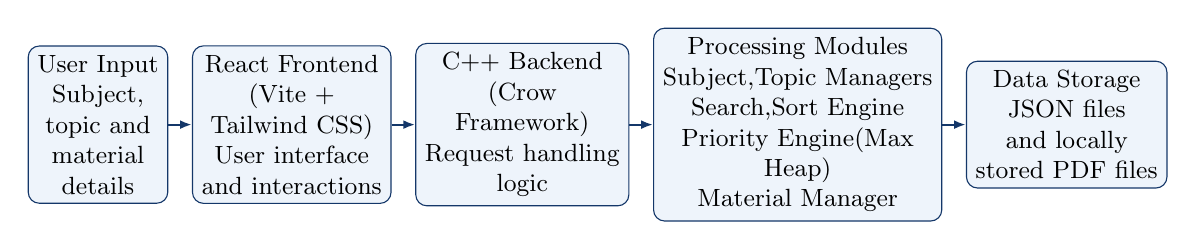
\begin{tikzpicture}[
node distance=3mm,
box/.style={
rectangle,
rounded corners,
draw=GEUBlue,
fill=GEULightBlue,
minimum width=1.5cm,
minimum height=9mm,
align=center,
font=\small
},
arrow/.style={
-{Latex[length=1.5mm]},
thick,
draw=GEUBlue
}
]

\node[box] (a) {User Input \\Subject, \\topic and \\material \\details};
\node[box,right=of a] (b) {React Frontend\\ (Vite + \\Tailwind CSS)\\User interface\\ and interactions};
\node[box,right=of b] (c) {C++ Backend\\ (Crow \\Framework)\\Request handling \\logic};
\node[box,right=of c] (d) {Processing Modules\\Subject,Topic Managers\\ Search,Sort Engine\\Priority Engine(Max\\Heap)\\ Material Manager};
\node[box,right=of d] (e) {Data Storage\\JSON files\\ and locally \\stored PDF files};

\draw[arrow] (a)--(b);
\draw[arrow] (b)--(c);
\draw[arrow] (c)--(d);
\draw[arrow] (d)--(e);

\end{tikzpicture}

\end{center}

\vspace{4mm}

\begin{columns}[T,totalwidth=\textwidth]

\column{.48\textwidth}
\vspace{-0.8cm}
\textbf{\color{GEUBlue}Major Components}

\begin{itemize}\itemsep2pt
    \item \placeholder{React-based frontend interface.}
    \item \placeholder{C++ Crow backend }
    \item \placeholder{OOP managers and DSA-based processing engines.}
    \item \placeholder{JSON persistence and local PDF storage.}
\end{itemize}

\column{.48\textwidth}
\vspace{-0.7cm}
\textbf{\color{GEUBlue}System Flow}

\begin{itemize}\itemsep2pt
    \item \placeholder{Input: User interacts through the React interface.}
    \item \placeholder{Processing: C++ backend handles requests and applies business logic and DSA algorithms.}
    \item \placeholder{Storage: Records are saved in JSON files and PDFs in local storage.}
\end{itemize}

\end{columns}

\vfill
\end{frame}

% ============================================================
% SLIDE 7
% ============================================================
\begin{frame}{Final Technology Stack}

\begin{columns}[T,totalwidth=\textwidth]

\column{.48\textwidth}

\begin{block}{Software / Technologies}
\begin{itemize}\itemsep2pt
    \item Programming: \placeholder{ C++}
    \item Framework: \placeholder{React, Vite, Tailwind CSS, Crow}
    \item Database/Storage: \placeholder{JSON file-based storage}
    \item Libraries/APIs: \placeholder{nlohmann/json, Crow REST APIs}
    \item OS/Platform: \placeholder{Windows 11}
\end{itemize}
\end{block}

\column{.48\textwidth}

\begin{block}{Development Infrastructure}
\begin{itemize}\itemsep2pt
    \item IDE: \placeholder{Visual Studio Code}
    \item Version Control:GitHub
    \item Testing Tools: \placeholder{CMake build, npm build, API testing}
    \item Deployment: \placeholder{Localhost-based development environment}
    \item Other Tools: \placeholder{Node.js, npm}
\end{itemize}
\end{block}

\end{columns}

\vfill
\end{frame}

% ============================================================
% SLIDE 8
% ============================================================
\begin{frame}{Implementation of PBL Course Concepts}

\scriptsize

\begin{center}

\renewcommand{\arraystretch}{1.25}

\begin{tabularx}{.98\textwidth}
{@{}>{\bfseries}p{2.8cm}X p{2.8cm}@{}}

\toprule
Course & Concepts Actually Implemented & Project Module\\
\midrule

Data Structures in C &
\placeholder{Arrays, vectors, hashing using unordered\_map, custom Max Heap, Linear Search, Binary Search, Merge Sort} &
\placeholder{Search and Sort Engine, Priority Engine}\\

OOPs with C++ &
\placeholder{Classes, Objects, Encapsulation, Constructors, Getters/Setters, } &
\placeholder{Subject, Topic, StudyMaterial and Manager classes }\\

\midrule


\end{tabularx}

\end{center}

\vfill


\end{frame}

% ============================================================
% SLIDE 9
% ============================================================
\begin{frame}{Module-Wise Final Implementation}

\scriptsize

\begin{center}

\renewcommand{\arraystretch}{1.35}

\begin{tabularx}{.96\textwidth}
{@{}p{2.4cm}X p{2.0cm}p{2.0cm}@{}}

\toprule
\textbf{Module} &
\textbf{Implementation} &
\textbf{Responsible} &
\textbf{Status}\\
\midrule

\placeholder{Subject Management and Search\/Sort } &
\placeholder{Subject CRUD operations, Linear Search, Binary Search and Merge Sort} &
\placeholder{Rehman Ullah Khan} &
Completed\\

\placeholder{Max Heap and Priority Engine} &
\placeholder{Custom Max Heap implementation and weighted priority calculation for recommendations. } &
\placeholder{Manan Lohni } &
Completed\\

\placeholder{Topic Management and Material Management } &
\placeholder{Topic CRUD operations and PDF upload, viewing, downloading and management.} &
\placeholder{Dipanshu Sirohi } &
Completed\\

\placeholder{Integration and DSA Visualization} &
\placeholder{Frontend-backend integration, testing, debugging and basic DSA visualizations.} &
\placeholder{ All Team Members} &
Completed\\

\bottomrule

\end{tabularx}

\end{center}

\vspace{1mm}

\begin{center}
\colorbox{GEULightBlue}{
\parbox{.65\textwidth}{
\centering
\textbf{Final Project Completion:}
\placeholder{100\%}
}}
\end{center}

\vfill



\end{frame}

% ============================================================
% SLIDE 10
% ============================================================
\begin{frame}{Working System / Prototype Demonstration}

\begin{columns}[T,totalwidth=\textwidth]

\column{.43\textwidth}
\vspace{-0.8cm}
\textbf{\color{GEUBlue}Major Working Features}

\begin{itemize}\itemsep3pt
    \item \placeholder{Subject and Topic Management: Add, edit, delete and manage subjects and topics with semester and exam-date details.}
    \item \placeholder{Smart Recommendations: Generate priority-based topic recommendations using a weighted formula.}
    \item \placeholder{Study Material Management: Upload, view, download, replace and delete PDF materials linked to subjects and topics.}
\end{itemize}

\column{.53\textwidth}

\begin{block}{System Screenshot / Output}

\centering
\vspace{11mm}

\placeholder{
Insert screenshot of final working system
}

\vspace{11mm}

\end{block}

\end{columns}

\vfill



\end{frame}

% ============================================================
% SLIDE 11
% ============================================================
\begin{frame}{Data / Database / Backend Implementation}

\begin{columns}[T,totalwidth=\textwidth]

\column{.48\textwidth}
\vspace{-0.8cm}
\textbf{\color{GEUBlue}Data / Database}

\begin{itemize}\itemsep3pt
    \item \placeholder{Database: JSON file-based storage; PDFs stored locally.}
    \item \placeholder{Schema / Data Structure: Separate JSON records for Subjects, Topics and Study Materials.}
    \item \placeholder{Important Entities: Subject, Topic and StudyMaterial.}
    \item \placeholder{Storage / Retrieval: C++ file handling with nlohmann/json for reading and writing records}
\end{itemize}

\column{.48\textwidth}
\vspace{-0.8cm}
\textbf{\color{GEUBlue}Backend / Core Logic}

\begin{itemize}\itemsep3pt
    \item \placeholder{Core Processing: C++17 backend using Crow HTTP framework.}
    \item \placeholder{API / Service: REST APIs exchange data with the React frontend using JSON.}
    \item \placeholder{Algorithm / Logic: Linear Search, Binary Search, Merge Sort and weighted priority calculation using a custom Max Heap.}
    \item \placeholder{Authentication / Security: User authentication is not implemented.}
\end{itemize}

\end{columns}

\vfill

\end{frame}

% ============================================================
% SLIDE 12
% ============================================================
\begin{frame}{Testing \& Validation}

\scriptsize

\begin{center}

\renewcommand{\arraystretch}{1.35}

\begin{tabularx}{.96\textwidth}
{@{}p{2.0cm}X X p{1.4cm}@{}}

\toprule
Test Type &
Expected Result &
Observed Result &
Status\\
\midrule

\placeholder{Unit Testing} &
\placeholder{ Individual modules should perform their intended operations correctly.} &
\placeholder{Subject, topic, search/sort and priority logic tests passed. } &
Pass\\

\placeholder{Integration Testing} &
\placeholder{Frontend, backend and APIs should communicate correctly.} &
\placeholder{API communication and Vite proxy tests passed.} &
Pass\\

\placeholder{System Testing} &
\placeholder{Complete application should build and run without major errors.} &
\placeholder{C++ backend and React production builds completed successfully. } &
Pass\\

\placeholder{Persistence Testing} &
\placeholder{ Data should remain available after application restart.} &
\placeholder{JSON persistence and restart tests passed. } &
\placeholder{Pass}\\

\bottomrule

\end{tabularx}

\end{center}

\vspace{3mm}




\end{frame}

% ============================================================
% SLIDE 13
% ============================================================
\begin{frame}{Results \& Performance Analysis}

\begin{columns}[T,totalwidth=\textwidth]

\column{.48\textwidth}
\vspace{-0.8cm}
\textbf{\color{GEUBlue}Key Results}

\begin{itemize}\itemsep3pt
    \item \placeholder{Functional Modules: All finalized modules implemented and integrated successfully.}
    \item \placeholder{Build Verification: C++ backend and React frontend production builds completed successfully.}
    \item \placeholder{Automated Testing: All Stage 7 automated tests passed.
}
    \item \placeholder{Data Persistence: Subject, topic and material records remained available after application restart in persistence tests.}
\end{itemize}

\column{.48\textwidth}

\begin{block}{Graph / Result Evidence}

\centering
\vspace{10mm}

\placeholder{
Insert graph / chart / result screenshot
}

\vspace{10mm}

\end{block}

\end{columns}

\vfill


\end{frame}

% ============================================================
% SLIDE 14
% ============================================================
\begin{frame}{GitHub Repository \& Development Evidence}

\begin{columns}[T,totalwidth=\textwidth]

\column{.45\textwidth}

\textbf{\color{GEUBlue}Repository Details}

\begin{itemize}\itemsep3pt
    \item Repository: \placeholder{https://github.com/Rehman-9/PBL\_GEU}
    \item Branch: \placeholder{main}
    \item README.md: \placeholder{Updated}
    \item Contributors: \placeholder{All members}
    \item Documentation: \placeholder{Available}
\end{itemize}

\column{.51\textwidth}

\textbf{\color{GEUBlue}Development Evidence}

\begin{itemize}\itemsep3pt
    \item \placeholder{Regular commits-32}
    \item \placeholder{Meaningful commit messages}
    \item \placeholder{Individual commits}
    \item \placeholder{Latest source code}
    \item \placeholder{Complete commit history}
\end{itemize}

\end{columns}

\vfill


\end{frame}

% ============================================================
% SLIDE 15
% ============================================================
\begin{frame}{Individual Contribution}

\scriptsize

\begin{center}

\renewcommand{\arraystretch}{1.35}

\begin{tabularx}{.96\textwidth}
{@{}p{1.8cm}p{1.8cm}X p{1.5cm}@{}}

\toprule
Member &
Role &
Final Technical Contribution &
Commits\\
\midrule

\placeholder{Rehman Ullah Khan} &
\placeholder{Team Lead Backend Developer } &
\placeholder{Implemented SubjectManager, Search and Sort Engine, JSON persistence and project integration.} &
\placeholder{15}\\

\placeholder{Manan Lohni} &
\placeholder{Backend and Algorithm Developer} &
\placeholder{Implemented Custom Max Heap and weighted Priority Engine and recommendation logic. } &
\placeholder{09}\\

\placeholder{Dipanshu Sirohi} &
\placeholder{DSA and Material Module Developer} &
\placeholder{Implemented Topic Manager and Study Material Management, including PDF upload, storage and retrieval. } &
\placeholder{09}\\


\bottomrule

\end{tabularx}

\end{center}

\vspace{3mm}


\end{frame}

% ============================================================
% SLIDE 16
% ============================================================
\begin{frame}{Challenges, Limitations \& Lessons Learned}

\begin{columns}[T,totalwidth=\textwidth]

\column{.48\textwidth}
\vspace{-0.8cm}
\textbf{\color{GEUBlue}Challenges \& Solutions}

\begin{itemize}\itemsep3pt
    \item \placeholder{Frontend–Backend Integration: Resolved API communication issues during integration.}
    \item \placeholder{Priority Calculation: Implemented weighted scoring with a custom Max Heap for accurate topic ranking.}
\end{itemize}

\vspace{1mm}

\textbf{\color{GEUBlue}Current Limitations}

\begin{itemize}\itemsep2pt
    \item \placeholder{No user authentication or multi-user access}
    \item \placeholder{Data is stored locally in JSON files and PDFs, rather than a centralized database or cloud storage.}
\end{itemize}

\column{.48\textwidth}
\vspace{-0.7cm}
\textbf{\color{GEUBlue}Technical Learning}

\begin{itemize}\itemsep3pt
    \item \placeholder{Improved understanding of C++ OOP, DSA implementation.}
    \item \placeholder{Learned React–C++ integration and JSON-based file handling.}
    \item \placeholder{Learning 3}
\end{itemize}

\vspace{1mm}

\textbf{\color{GEUBlue}Team Learning}

\begin{itemize}\itemsep2pt
    \item \placeholder{Improved collaboration through division of modules and integration.
}
    \item \placeholder{Developed practical problem-solving and project coordination skills.}
\end{itemize}

\end{columns}

\vfill



\end{frame}

% ============================================================
% SLIDE 17
% ============================================================
\begin{frame}{Final Outcomes, Applications \& Future Scope}

\begin{columns}[T,totalwidth=\textwidth]

\column{.32\textwidth}
\vspace{-0.7cm}
\textbf{\color{GEUBlue}Final Outcomes}

\begin{itemize}\itemsep3pt
    \item \placeholder{Developed a functional web-based study management system using React and C++.
}
    \item \placeholder{Implemented subject, topic and PDF material management.}
    \item \placeholder{Integrated searching, sorting and smart topic recommendations using a custom Max Heap.}
\end{itemize}

\column{.32\textwidth}
\vspace{-0.7cm}
\textbf{\color{GEUBlue}Applications}

\begin{itemize}\itemsep3pt
    \item \placeholder{Organizing academic subjects, topics and syllabus progress.
}
    \item \placeholder{Identifying important topics based on exam urgency and study requirements.}
    \item \placeholder{Managing study notes and PDF resources in one place.}
\end{itemize}

\column{.32\textwidth}
\vspace{-0.7cm}
\textbf{\color{GEUBlue}Future Scope}

\begin{itemize}\itemsep3pt
    \item \placeholder{Add user authentication and individual student accounts.}
    \item \placeholder{Introduce cloud-based storage and database integration.}
    \item \placeholder{Develop a personalized study planner with progress tracking and reminders.
}
\end{itemize}

\end{columns}

\vspace{5mm}

\begin{block}{Tangible Project Outcome}
\placeholder{
Mention whether the project resulted in a working prototype,
deployment, dataset, research work, technical solution or other
demonstrable outcome.
}
\end{block}

\end{frame}

% ============================================================
% SLIDE 18
% ============================================================
\begin{frame}{References \& Project Resources}

\begin{columns}[T,totalwidth=\textwidth]

\column{.53\textwidth}

\textbf{\color{GEUBlue}References}

\begin{enumerate}\itemsep3pt
    \item \placeholder{C++ Documentation – [cppreference.com]}
    \item \placeholder{React Documentation – [react.dev]}
    \item \placeholder{Crow C++ Framework – [crowcpp.org]}
    \item \placeholder{nlohmann/json Documentation – [json.nlohmann.me]}
    \item \placeholder{GeeksforGeeks – Data Structures and Algorithms concepts}
\end{enumerate}

\column{.43\textwidth}

\textbf{\color{GEUBlue}Project Resources}

\begin{itemize}\itemsep3pt
    \item GitHub: \placeholder{https://github.com/Rehman-
9/PBL\_GEU}
    \item Documentation: \placeholder{ Project README available in the GitHub repository}
\end{itemize}

\vfill

\begin{center}

\colorbox{GEUBlue}{
\parbox{.82\textwidth}{
\centering
\color{white}
\Large\textbf{Thank You}\\[1mm]
\normalsize Questions \& Discussion
}}

\end{center}

\end{columns}

\end{frame}

\end{document}
